\documentclass[journal,draftclsnofoot,onecolumn,12pt]{IEEEtran}
\usepackage{setspace}

\usepackage{amsthm,amssymb,graphicx,multirow,amsmath,color,amsfonts}%,ulem}
\usepackage[update,prepend]{epstopdf}
\usepackage[noadjust]{cite}
%\usepackage{ucs}
%s\usepackage[latin1]{inputenc}
\usepackage{tikz}
\usetikzlibrary{arrows,calc}		% Optional ticks libraries
\usepackage{bbm} % for \mathbbm{1}
\usepackage{pdfpages}
%\usepackage{flushend}
\usepackage{tabulary}
\usepackage{multirow}
\usepackage{comment}
\usepackage{lipsum}
\usepackage{float}
\usepackage{subcaption}

\usepackage{cite}

\usepackage{lettrine}

\theoremstyle{definition}
\newtheorem{defn}{Definition}[section]
\newtheorem{conj}{Conjecture}[section]
\newtheorem{exmp}{Example}[section]

\usepackage{array}
\usepackage{booktabs}
\setlength{\heavyrulewidth}{1.5pt}
\setlength{\abovetopsep}{4pt}


\usepackage{hyperref}
\usepackage{algorithm}

\usepackage{longtable,tabularx,tabulary}


\usepackage{remreset}
\usepackage{optidef}
\usepackage{listings}
\usepackage{enumitem}

\epstopdfsetup{update} % only regenerate pdf files when eps file is newer


\usepackage{array}
\newcolumntype{P}[1]{>{\centering\arraybackslash}p{#1}}

\usepackage{makecell}



\makeatletter
\newcommand{\onetagright}{\tagsleft@false}
\makeatother

%\usepackage{breqn}

% Colors
\def\chr#1{{\color{red}#1}}
\def\chb#1{{\color{blue} #1}}

\allowdisplaybreaks % Allows breaking of eqnarray over multiple pages (avoids unnecessary blanks in the document before eqnarray)

%%%%%%%%%%%%%%%%%%%%%%%%%%%%%%%%%%%%%%%%%



\doublespacing
\begin{document}
	\graphicspath{{./images/}}
	\title{Review on 5G New Radio \\}
	


	
	\author{ Mansour Naslcheraghi (1965148), Claudio (XXXXXX)\\Alex (XXXXXX), Maha (XXXXXX)\\ ELE6709 Final Project\\ Prof. Jean-François Frigon \\ \today 		
	}

	
	\maketitle
	\thispagestyle{empty}
	\pagestyle{empty}
	
	
	
	
	
%	\maketitle
	%\thispagestyle{empty}
	%\pagestyle{empty}
	
	%\begin{abstract}
	%%\lipsum[1]
	%\end{abstract}
	%
	%\begin{IEEEkeywords}
	%
	%\end{IEEEkeywords}
	
	\newpage
	\tableofcontents
	
	\newpage
%%%%%%%%%%%%%%%%%%%%%%%%%%%%%%%%%%%%%%%%%%%%%%%%%%%%%%%%%%%%%
\section{Introduction}
Goes here...
%%%%%%%%%%%%%%%%%%%%%%%%%%%%%%%%%%%%%%%%%%%%%%%%%%%%%%%%%%%%%




%%%%%%%%%%%%%%%%%%
\section{Radio Resource Management in 5G NR}
\label{sec:mansintro}
%%%%%%%%%%%%%%%%%%%
Resource management has always been a key part of designing cellular communications, especially when there are limitations on the available resources. In cellular communications, the term ``resource'', traditionally referred to spectrum and power. However, with the emergence of modern cellular networks along with the advent of new technologies, the term ``resource'' has gotten even more broad aspects; high demand for online computing services raised limitations on ``computing'' resources and hardware equipment along with required storage. Hence, nowadays, the term ``resource'' has much more broad aspects than that of the interpretations in the traditional cellular networks, e.g., 2G and 3G. Among those aforementioned terms, the term ``spectrum'' has always been at the center of designing concerns among all operators. Cellular networks sustained on their legs for decades by relying on so-called \textit{sweet spectrum}, which refers to frequency bands between 500 MHz and 3000 MHz. This frequency band is unique and due to long distance travel capability while providing meaningful transmissions of data, operators are paying billions of dollars to own part of this spot, especially between 500 MHz and 1000 MHz. One can compare this sweet spot with the ``location'' term in real estate business joke; the most important components of real estate are location, location, location! Skyrocketing increase in the number of users and tremendous demand on data traffic caused cellular network operators to face challenges in accommodating their users' needs with the satisfying Quality of Service (QoS). Fortunately, 5G New Radio (NR) unlocks much higher frequencies to support diverse end users with a variety of QoS requirements. While 5G NR promises high data rate and an ultra low latency, nevertheless, it does not come without challenges and cost. Achieving true 5G capacity requires massive installation of the equipment across the entire network as it requires utilizing mmWave spectrum. However, standardization units came across to an unanimous agreement that 5G should include the previous generations as the key part of the system, especially for the situations where a high coverage is needed, in which the sub-6 GHz would be good option, i.e., Fig. \ref{fig:sub6} illustrates the tradeoff between capacity and coverage with respect to different spectrum. As can be seen, the sweet spectrum is Sub-1 GHz, which is almost occupied by different operators. In the sequel, frame structure and numerology of 5G NR is briefly explained in subsection \ref{subsec:numerology_framestructure}, subsection \ref{subsec:slotformat} will go through the slot format in 5G NR. Subsection \ref{subsec:5Gscheduling} briefly introduces the scheduling mechanism in 5G NR, and subsection \ref{subsec:5GNR_num_RA} gives a brief glance on methodologies and challenges in 5G NR resource allocation with respect to different numerologies. 
\begin{figure}[!ht]
	\centering
	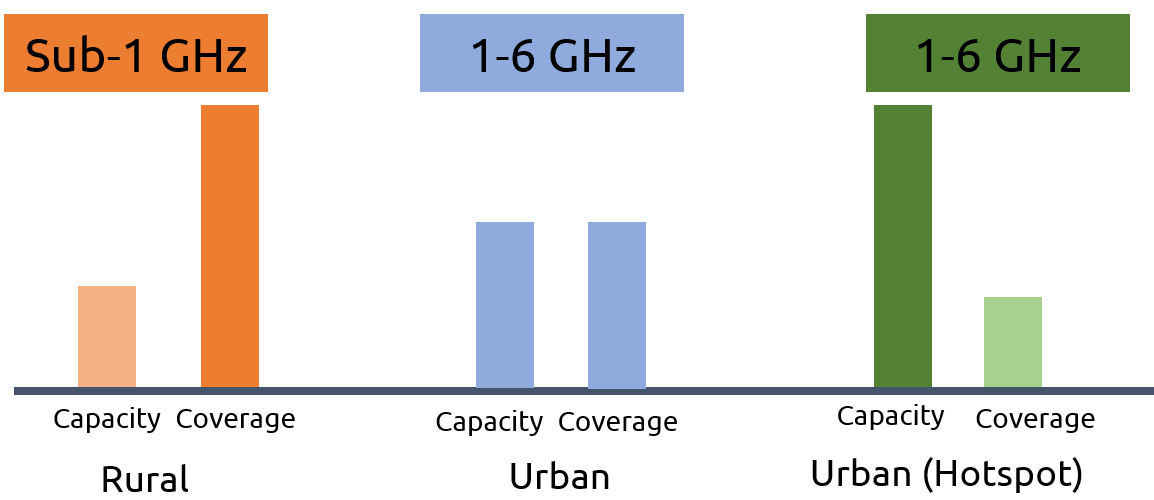
\includegraphics[width=0.55 \textwidth]{images/sub6-2.png}%\vspace{-6mm}
	\caption{Capacity and coverage of different spectrum.} 
	\label{fig:sub6}
\end{figure}
%%%%%%%%%%%%%%%%
\subsection{Numerology and frame Structure in 5G NR}
\label{subsec:numerology_framestructure}
%%%%%%%%%%%%%%%%
In contrast with the LTE cellular system, 5G NR brings more flexibility to accommodate massive number of users along with different service types and diverse Quality of Service (QoS) requirements. Beside variety of technologies in 5G, these capabilities are endowed by introducing new scalable resource partitioning called \textit{5G NR Numerologies}. While the Resource Blocks (RBs) in LTE system are composed of 12 subchannel each with always 15 KHz bandwidth (total $12\times180$ KHz per each RB), RBs in 5G NR, with the same number of subcarriers yet can have different bandwidth depending on the numerology configurations and the requirements of the target service of interest. The very fist introduction on the frame structure is delineated in Fig. \ref{fig:Numerology_RB} along with details in the associated table, in which the parameter $\mu$ accounts for the numerology type. Technically, an RB of 5G NR can have bandwidth of $2^{\mu}$ times of bandwidth of an RB in LTE. This means that $\mu = 0 $ accounts for the RB in the LTE system. In overall, an RB in 5G comprises of one timeslot and 12 subcarriers with Sub Carrier Spacing (SCS) of $2^{\mu} \times 15$ KHz. Hence, an RB can accommodate bandwidth from 150 KHz to 720 KHz depending on the values of $\mu$. Cyclic Prefix (CP) is the duration of the guard band. 
%\begin{table}[ht!]
%	\centering
%	\begin{tabular}{c|c|c|c|c|c}
%		SCS Index ($\mu$) & $\mu=0$ & $\mu=1$ & $\mu=2$ & $\mu=3$ & $\mu=4$ \\
%		\hline
%		Each SCS (in KHz) & 15 & 30 & 60 & 120 & 240 \\
%		Each RB's BW (in KHz) & 180 &  360  & 720 & 1440 & 2880\\
%	\end{tabular}
%	\caption{5G NR Numerology}
%	\label{tab:numerology}
%\end{table}
\begin{figure}[!ht]
	\centering
	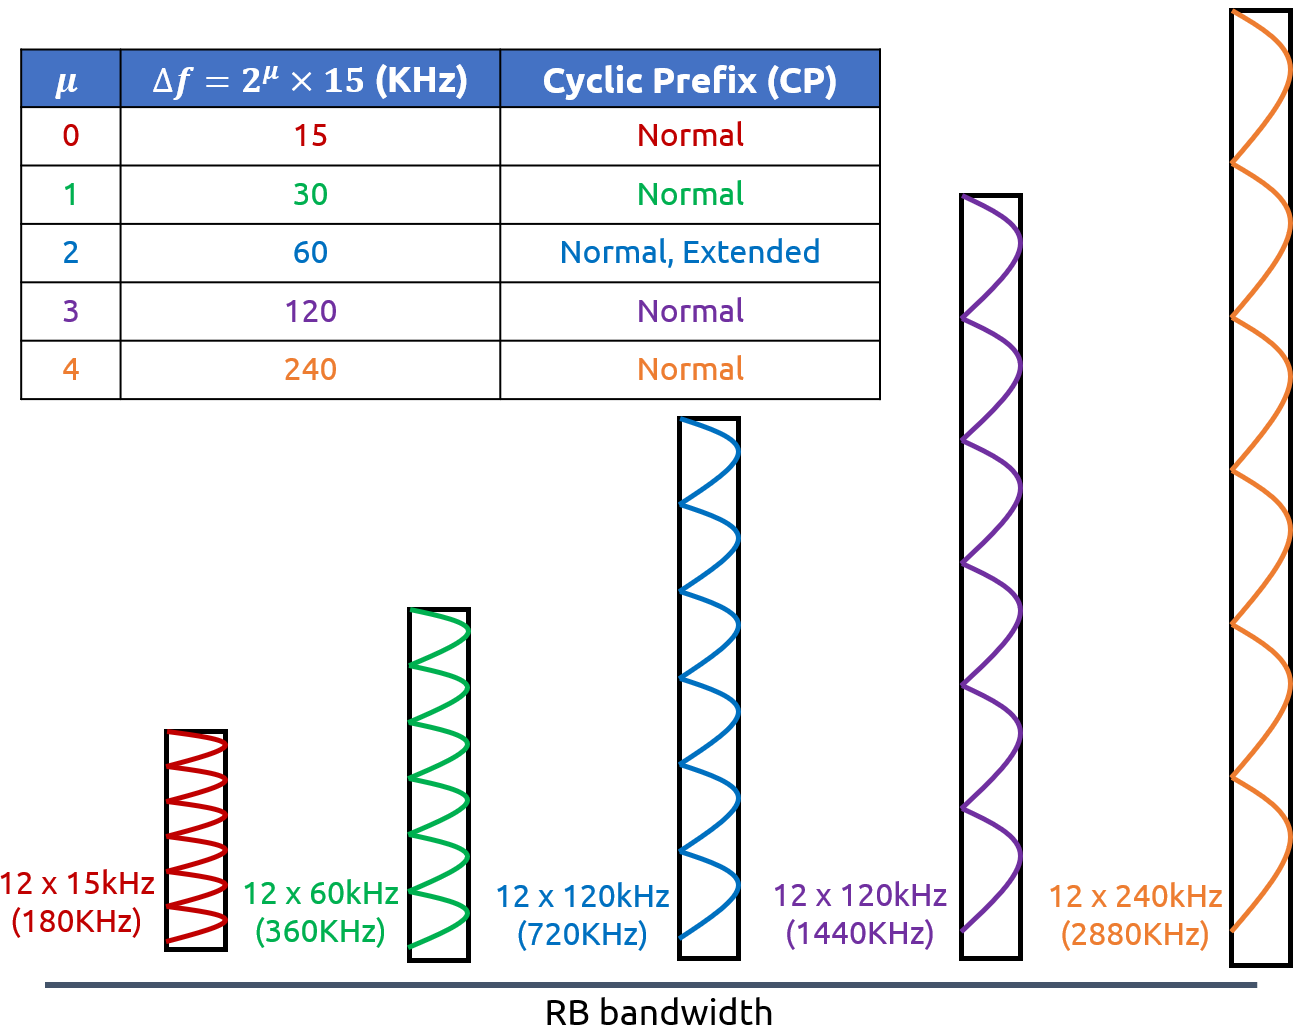
\includegraphics[width=0.7 \textwidth]{images/Numerology_RB.PNG}%\vspace{-6mm}
	\caption{Bandwidth of RBs for different numerologies.} 
	\label{fig:Numerology_RB}
\end{figure}

Fig. \ref{fig:numerology}(a) illustrates the slot-based frame for given numerologies. As can be seen, for every step of shrinking time slot, we have more bandwidth available. It is also possible to divide each time slot into minislots as delineated in Fig. \ref{fig:numerology}(b) to satisfy QoS requirements of delay-critical services such as ultra Reliable Low Latency Communications (uRLLC). This flexibility is endowed by splitting symbols between minislots, which means that less symbols can be transmitted within a short time to meet stringent latency requirement of some mission-critical applications, e.g., Safety-Oriented Applications of the Cellular Vehicle-to-Everything (C-V2X) communications. Observations on Fig. \ref{fig:numerology} implies that, given the type of the application, one can allocate resources by i) spanning in time domain while considering fix frequency band or ii) spanning in frequency domain while considering fix time duration. In the other words, one can allocate single minislot along with its spanning frequency domain available within each minislot or can allocate a frequency band by considering more than one minislot in the same frequency band. For example, for a mission-critical applications, it is more crucial to deliver/retrieve data within an stringent latency deadline, which means that the spanning in frequency domain by considering small minislot is more appropriate for this type of application. However, for an smart metering device, it is more efficient to allocate less frequency yet within more consecutive or nonconsecutive minislots. Table \ref{tab:time_duration_slots} shows the values for the time duration pf time-slots along with the number of slots to be accommodated within a subframe. Standardization organizations such as third Generation Partnership Project (3GPP) came across to new rules to utilize mmWave and sweet spectrum in more systematic way by using mixed numerology resource allocation, in which different numerologies can be utilized for different applications \cite{5GNR_MAC,5GNR_Mod,5GNR_PHY}.  
\begin{figure}[!ht]
	\centering
	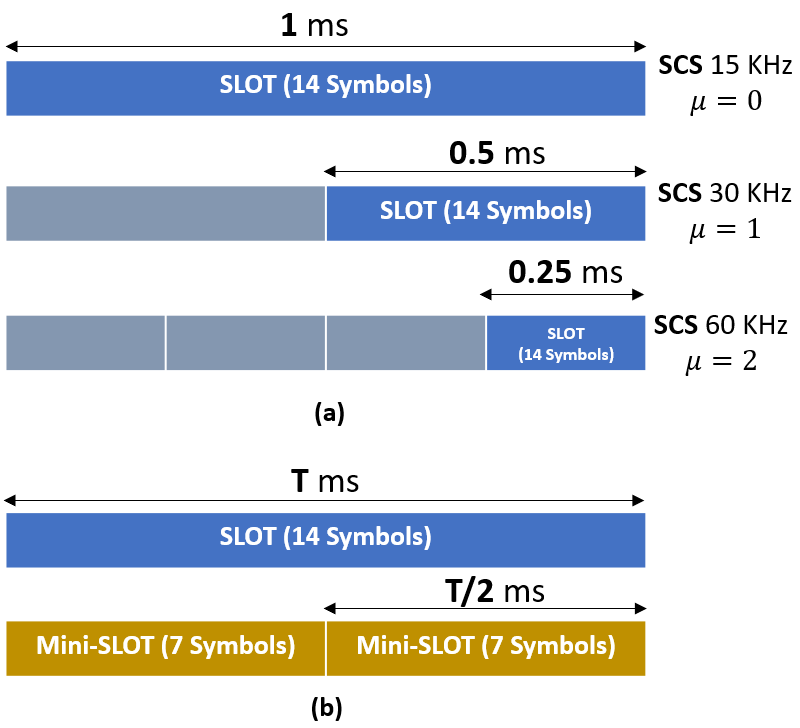
\includegraphics[width=0.5 \textwidth]{images/Numerology.png}%\vspace{-6mm}
	\caption{Demonstration of (a) Slot-Based subframe and (b) Mini-Slot based subframe.} 
	\label{fig:numerology}
\end{figure}
\begin{table}[ht!]
	\centering
	\begin{tabular}{c|c|c|c|c|c}
		SCS Index ($\mu$) & $\mu=0$ & $\mu=1$ & $\mu=2$ & $\mu=3$ & $\mu=4$ \\
		\hline
Time duration of time-slot (in ms) & 1 & 0.5 & 0.25 & 0.125 & 0.0625 \\
Slots per subframe & 1 & 2 & 4 & 8 & 16  
	\end{tabular}
	\caption{5G NR Numerology}
	\label{tab:time_duration_slots}
\end{table}
Not all numerologies are suitable for all frequency bands. Table \ref{tab:SCS_sub6_mmWave} shows the allowed SCS values for the important bands of sub-6 GHz and above 6 GHz.
\begin{table}[!h]
	\centering
	\begin{tabular}{c|c|c}
		& Sub-6 GHz & mmWave \\
		\hline
		SCS (MHz) & 5/10/15/20/25/40/50/60/80/100 & 50/100/200/400 \\
		BW per carrier (KHz) &  15/30/60  &  60/120/240 \\
	\end{tabular}
	\caption{Sub-6 GHz and mmWave SCS and BW per carrier \cite{5GNR_PHY}}
	\label{tab:SCS_sub6_mmWave}
\end{table}
%%%%%%%%%%%%%%%%%%%%%%%%%%%%%%%%%%%%
\subsection{Slot Format and Time Duration}
\label{subsec:slotformat}
%%%%%%%%%%%%%%%%%%%%%%%%%%%%%%%%%%%%
 Fig. \ref{fig:Numerology_frame_subframe} demonstrates the bandwidth versus time duration for different numerologies along with the number of slots per frame ($N_{\rm slot}^{\rm frame, \mu}$ in the second column of table in Fig. \ref{fig:Numerology_frame_subframe}) and the number of slots per subframe ($N_{\rm slot}^{\rm subframe, \mu}$ in the last column of table in Fig. \ref{fig:Numerology_frame_subframe}, for the given numerology parameter $\mu$. The frame and subframe structure has been delineated in more details in Fig. \ref{fig:Numerology_FrameStructure}. The length of one radio frame is always 10 ms and the length of a subframe is always 1 ms, regardless of the numerology. Also, the number of symbols within each slot is always 14 symbols unless the structure is based on minislot (as in Fig. \ref{fig:numerology}(b)).   
\begin{figure}[!ht]
	\centering
	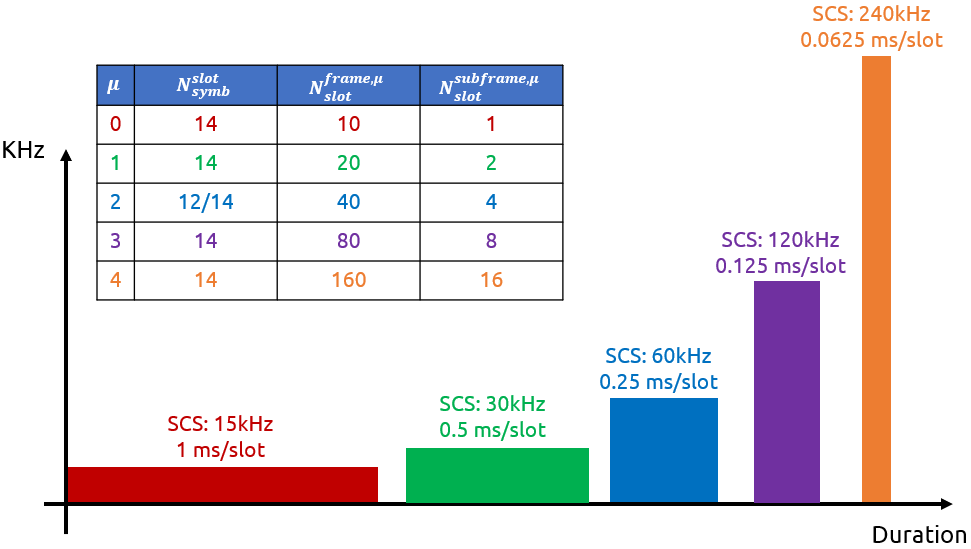
\includegraphics[width=0.8 \textwidth]{images/Numerology_frame_subframe.PNG}%\vspace{-6mm}
	\caption{Relationship between the duration and and the number of slots within a frame.} 
	\label{fig:Numerology_frame_subframe}
\end{figure}
\begin{figure}[!ht]
	\centering
	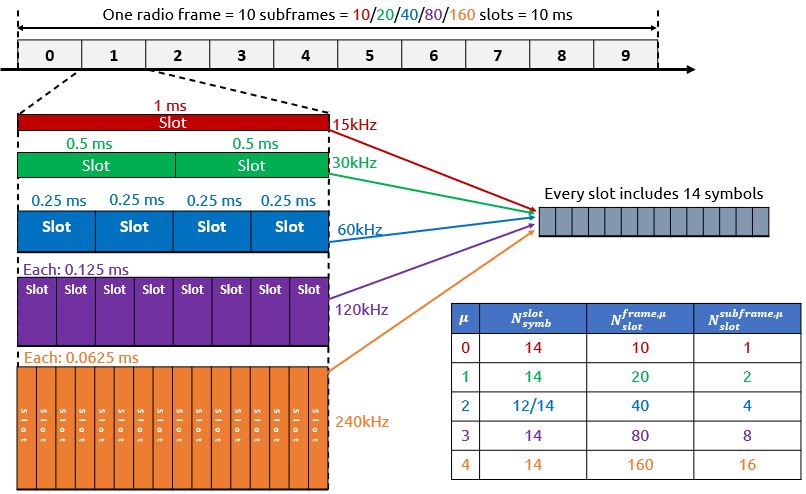
\includegraphics[width=0.8 \textwidth]{images/Numerology_FrameStructure.PNG}%\vspace{-6mm}
	\caption{Frame Structure based on different numerologies.} 
	\label{fig:Numerology_FrameStructure}
\end{figure} 
%%%%%%%%%%%%%%%%%%%%%%%%%%%%%%%%%%%
\section{Which Numerology and When: Resource Allocation in 5G NR}
\label{sec:5GNR_num_RA}
%%%%%%%%%%%%%%%%%%%%%%%%%%%%%%%%%%%
The unique capability of resource management in 5G NR in comparison with the previous generations, is to utilize different numerologies and even mixed-numerology resource allocation depending on many conditions in the end-to-end resource allocation procedures. 5G NR is flexible of choosing appropriate numerology to fit the dynamic conditions. It is unlikely to choose a high bandwidth RB numerology for the communications that desire better coverage, to choose a low bandwidth numerology for the communications that a very low latency is required. In fact, since 5G system is more than a infrastructure for the traditional mobile communications, system should be able to adopt different type of RBs for different purposes. There are many factors involved in such decisions and Fig. \ref{fig:num_cellsize_latency} sketches the relationship between a a few factors. As can be seen, cell-size achievable latency are strongly related to the carrier frequency. It is noted that the low latency can also be achieved in larger cells using wider subcarrier spacing. However, this may incur a performance penalty in terms of reliability or throughput \cite{num_cellsize_latency}.  
\begin{figure}[H]
	\centering
	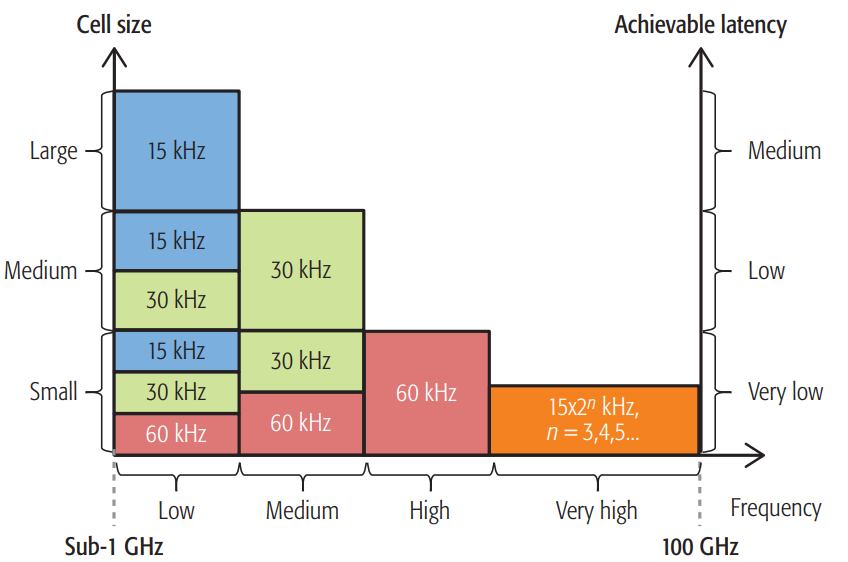
\includegraphics[width=0.65 \textwidth]{images/num_cellsize_latency.PNG}%\vspace{-6mm}
	\caption{OFDM numerology design for wide range of carrier frequencies,
		deployment types, and application latency requirements using regular slots \cite{num_cellsize_latency}.} 
	\label{fig:num_cellsize_latency}
\end{figure}
Fig. \ref{fig:optimalFsc_vs_Doppler} illustrates the optimal subcarrier frequency ($f_{\rm sc}$ (KHz)) and optimal number of symbols $n_{\rm D}$ versus Doppler shift (Hz) \cite{Numerology_mobility}. Simulation results in \cite{Numerology_mobility} demonstrate that in higher mobility conditions with high SNR regimes, the choice of numerology is much more important than that of the conditions where there is lower mobility, and the choice of numerology has a major impact on the achievable \textit{effective capacity} \cite{effective_capacity}. Technically, in 5G NR, numerology design is based on the service type, service requirements, and user requirements, and this is what makes 5G quite different from the previous generations. Table \ref{tab:service_req_num} shows the key requirements for different service types \cite{numerology_flex_service_user_req}. For instance, uRLLC service with low latency requires shorter Transmission Time Interval (TTI), which is the duration of the transmission on the radio link. Or, for the uRLLC service type with high reliability, time duration of the Cyclic Prefix ($T_{\rm CP}$) should be long, as it is necessary to deal with the Inter Symbol Interference (ISI) as well as intra-symbol interference. The guard time should be long enough to avoid overlap between the symbols in the frequency domain. Table \ref{tab:user_req_num} shows the requirements to deal with the important constraints for different impairment types, i.e., channel and RF hardware. This table also implies that there are many factors in designing the desired numerology to meet user requirements. For instance, we can combat larger Doppler shift by designing having larger $\Delta f$, which is larger subcarrier spacing. This argument well fits with the results demonstrated in Fig. \ref{fig:optimalFsc_vs_Doppler} obtained by \cite{Numerology_mobility}.   
\begin{figure}[!ht]
	\centering
	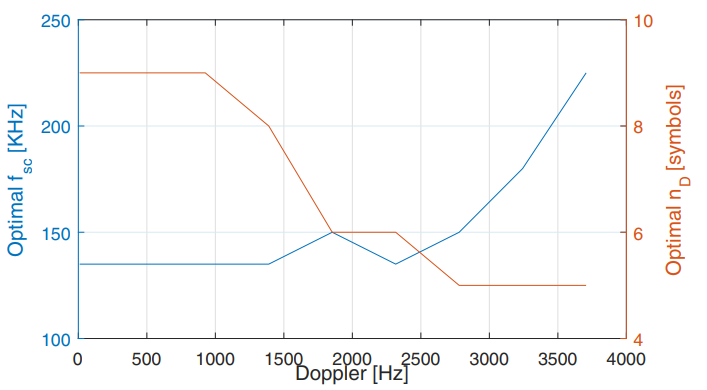
\includegraphics[width=0.6 \textwidth]{images/optimalFsc_vs_Doppler.PNG}%\vspace{-6mm}
	\caption{Optimal subcarrier spacing frequency versus Doppler effect \cite{Numerology_mobility}} 
	\label{fig:optimalFsc_vs_Doppler}
\end{figure}
\begin{table}[!h]
	\centering
	\caption{Service requirements and their effects numerology parameters \cite{numerology_flex_service_user_req}. }
	\label{tab:service_req_num}
	\begin{tabular}{|c|c|c|c|c|c|c|}
		\hline
		\multirow{2}{*}{\begin{tabular}[c]{@{}c@{}}Service \\ Type\end{tabular}} & \multirow{2}{*}{\begin{tabular}[c]{@{}c@{}}Key \\ Requirement\end{tabular}} & \multicolumn{5}{c|}{If any, key necessities for numerology design}            \\ \cline{3-7} 
		&                                                                             & $\eta_{\rm spectrul}$ & $\Delta f$ & \# of subcarriers & TTI   & $T_{\rm CP}$ \\ \hline
		\multirow{2}{*}{eMBB}                                                    & High Throughput                                                             & High                  &            &                   &       &              \\ \cline{2-7} 
		& High Data Rate                                                              & High                  &            &                   &       &              \\ \hline
		\multirow{2}{*}{mMTC}                                                    & \begin{tabular}[c]{@{}c@{}}Support for \\ small data bursts\end{tabular}    &                       & Large      &                   &       &              \\ \cline{2-7} 
		& High energy efficiency                                                      &                       &            & Low               &       &              \\ \hline
		\multirow{2}{*}{uRLLC}                                                   & Low latency                                                                 &                       &            &                   & Short &              \\ \cline{2-7} 
		& High reliability                                                            &                       & Large      &                   &       & Long         \\ \hline
	\end{tabular}
\end{table}
\begin{table}[!h]
	\centering
	\caption{User requirements and their effects numerology parameters \cite{numerology_flex_service_user_req}.}
	\label{tab:user_req_num}
	\begin{tabular}{|c|c|c|c|c|c|c|}
		\hline
		\multirow{2}{*}{\begin{tabular}[c]{@{}c@{}}Impairment\\ Type\end{tabular}} & \multirow{2}{*}{\begin{tabular}[c]{@{}c@{}}Important\\ Constraint\end{tabular}} & \multicolumn{5}{c|}{If any, key necessities for numerology design}          \\ \cline{3-7} 
		&                                                                                 & $\eta_{\rm spectrul}$ & $\Delta f$ & \# of subcarriers & TTI & $T_{\rm CP}$ \\ \hline
		\multirow{3}{*}{Channel}                                                   & Doppler                                                                         &                       & Large      &                   &     &              \\ \cline{2-7} 
		& Multipath                                                                       &                       &            &                   &     & Long         \\ \cline{2-7} 
		& pathloss                                                                        &                       &            & Low               &     &              \\ \hline
		\multirow{3}{*}{RF Hardware}                                               & Phase noise                                                                     &                       &            &                   &     &              \\ \cline{2-7} 
		& Frequency offset                                                                &                       & Large      &                   &     &              \\ \cline{2-7} 
		& PA none-Linearity                                                               &                       & Large      & Low               &     &              \\ \hline
	\end{tabular}
\end{table}
Coexistence of different numerologies has advantages and disadvantages, which forms the basis of the next subsection. However, before moving to make discussion on challenges, let us take a quick review on the resource allocation in frequency and time domain based on 5G NR. 
\subsection{Time and Frequency Domain Resource Allocation in 5G NR}
\label{subsec:time_freq_allocation}
According to specifications in \cite{3GPP_Rel17}, here is the brief summary of time and frequency domain resource allocation in 5G NR. 
\paragraph{Time-Domain} 5G NR supports the one-slot, minislot, and multiple slot resource allocation. Minislot can accommodate 2, 4, or 7 OFDM symbols. Duration depends on the numerology and SCS. Namely, the higher SCS, leads to lower duration (as illustrated in Fig. \ref{fig:numerology}), which is suitable for the uRLLC transmissions. However, the downside of the lower duration is that it also impacts the CP, which can cause lower coverage. That's why such implementation is much useful for compact cells. 5G gives symbol-level scheduling possibility. While in the LTE system, everything is reffered to TTI, which is equal to 1 ms. Hence, with 5G, this procedure can be very flexible.   
\paragraph{Frequency-Domain} Even though the RB structure, as explained in the previous sections, is similar to LTE (12 subcarriers), however, while 5G supports the active types within the LTE system, it also brings more flexibility. There are two types of resource allocation in frequency domain; \textit{Type 0}: this type is none-distributed allocation in frequency domain. RBs forms RB Groups (RBGs), in which the number of RBs per group depends on the bandwidth. This type utilizes none-interleaved mapping between virtual RBs and physical RBs. \textit{Type 1}: This is a distributed resource allocation and the interleaving is an open option, which can be either utilized or ignored. \textit{Dynamic Switching}: making switch between two types and this capability is new in 5G NR and LTE system does not support it. It allows to make switch between two types depending on the conditions. In practice, the type is determined by the Downlink Control Information (DCI). 
%%%%%%%%%%%%%%%%%%%%%%%%%%%%%%%%%%%
\subsection{Some Challenges and Ongoing Efforts to Resolve Them}
\label{subsec:challenges}
%%%%%%%%%%%%%%%%%%%%%%%%%%%%%%%%%%% 
Even though 5G NR provides highly flexible numerology for the resource allocation, nevertheless, there are some drawbacks using this technology. We already heard terms Inter Symbol Interference (ISI) and Inter Carrier Interference (ICI). The term Inter Numerology Interference (INI) is a new type of interference comes with 5G NR numerology, which induces interference between multiple numerologies due to coexistence of multiple numerologies, which deteriorates the system performance. In the sequel, some efforts to resolve this issue are highlighted. 

\subsubsection{Interference Pattern Derivation}
 Existing works, to name a few, \cite{numerology_INI, numerology_INI2, numerology_INI_MIMO}, recently aimed to deal with this issue. By dividing the INI into a dominant deterministic part and an equivalent noise part, authors in \cite{numerology_INI} proposed scheme to cancel the dominant interference, and the residual interference power is utilized as effective noise variance for the calculation of log-likelihood ratios for bits. An investigation is done by \cite{numerology_INI2} to obtain the interference pattern and the results reveals that the variance of interference energy increases due to the difference in SCS. By deriving radiation pattern in massive MIMO-OFDM downlink system in \cite{numerology_INI_MIMO}, it has been shown that by utilizing the proposed precoding, INI appears only in frequency selective channels. Besides, the transmission of users using numerology with large SCS is always with the best quality. 



%The analytical expression of the INI power is derived as a function of the channel frequency response of interfering subcarrier, the spectral
%distance separating the aggressor and the victim subcarrier, and the overlapping windows generated by the interferer's transmitter windows and the victim's receiver window. Based on the derived INI power expression, a novel INI cancelation scheme is proposed by dividing the INI into a dominant deterministic part and an equivalent noise part. A soft-output ordered successive interference cancelation (OSIC) algorithm is proposed to cancel the dominant interference, and the residual interference power is utilized as effective noise variance for the calculation of log-likelihood ratios for bits. \cite{numerology_INI}.


%Mixed numerology SS systems suffer from inter-numerology interference (INI). We first derive the interference pattern and find that the variance of interference energy increases due to the difference in SCS. This increase in variance negatively affects decoding performance, since the interference energy is unbalanced between subcarriers \cite{numerology_INI2}.


%Then, we analyse the inter-numerology interference (INI) and derive the theoretical expressions of its radiation pattern in massive MIMO-OFDM downlink systems. We demonstrate that by using the proposed precoding scheme and considering two groups of users using two different numerologies, INI appears only in frequency selective channels. Besides, the transmission of users using numerology with large subcarrier spacing (SCS) is always with the best quality, only users using the numerology with small SCS suffer from INI. In that case, INI increases due to the difference in SCS, channel selectivity and power allocation \cite{numerology_INI_MIMO}.



\subsubsection{Filtering \& Guard Band Design}To name a few, \cite{num_interference_f_OFDMA, num_CP_optimization,num_guardband_reduction,num_guardband_reduction3,num_guardband_reduction2}. It has been shown in \cite{num_interference_f_OFDMA} that a filtered OFDM (F-OFDMA) system accommodates the coexistence of the mixed numerologies better than that of the none-filtered counterpart. Combining F-OFDM with MIMO in \cite{num_CP_optimization} further improves the system capacity. The key challenge is to choose (optimize) an appropriate CP length such that it consumes less amount of time and at the same time, combats ISI and ICI. The F-OFDM MIMO system with the optimized CP outperforms conventional OFDM system. Designing an spectral-usage efficient Guard Band (GB) is targeted in \cite{num_guardband_reduction}, which reduces the GB spectrum utilization by \%50 while achieving the same error rate as the conventionally implemented GB. The follow-up work \cite{num_guardband_reduction3} put the same idea yet by analyzing INI and deriving outage probability of each subcarrier. Finally, the authors in \cite{num_guardband_reduction2} optimized the GBs in the adjacent bands as shown in Fig. \ref{fig:adaptive_GB}, with respect to SCS, service requirement, and power offset between numerologies.     
\begin{figure}[!ht]
 	\centering
 	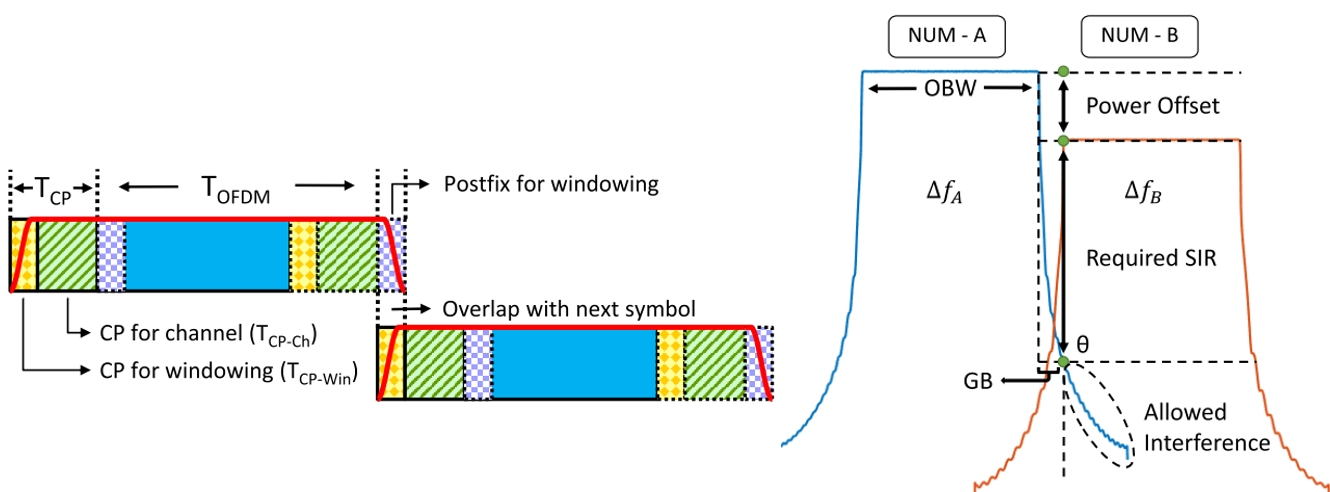
\includegraphics[width=0.7 \textwidth]{images/adaptive_GB.PNG}%\vspace{-6mm}
 	\caption{Adaptive guardband design in \cite{num_guardband_reduction2}  } 
 	\label{fig:adaptive_GB}
\end{figure}
 
 
  
 % the level of InterNI is quantified by the developed analytical metric, which is expressed as a function of several system parameters. It is also demonstrated that a filtered-OFDM system better accommodates the coexistence of mixed numerologies \cite{num_interference_f_OFDMA}.
 
 
%Filtered-orthogonal frequency division multiplexing (F-OFDM) is a potential waveform which uses sub-band filtering to support multi-numerologies in the future 5G systems. It is a future trend to combine F-OFDM with MIMO to further improve the system capacity. However, when employing different numerologies, a long filter length is needed to suppress severe inter-user interference (IUI) caused by various symbol duration in time domain, which causes inter-symbol interference (ISI) and inter-carrier interference (ICI) at the same time. Longer CP is helpful to resist the effect of multipath and filter responds but will waste more time resource. In order to reduce ISI and ICI while improving the spectrum efficiency, we propose a CP optimization model based on theoretical derivation of ISI, ICI and IUI for downlink MIMO F-OFDM system. The simulation results show that the ISI and ICI decrease as CP gets longer, while the spectrum efficiency is improved based on the proposed CP optimization model and outperforms traditional OFDM \cite{num_CP_optimization}.
 
 
% The existence of inter-numerology interference (INI)
% is a major drawback for the flexible multi-numerology frame
% structure proposed for the upcoming fifth generation New Radio (5G-NR). Insertion of a guard band (GB) between adjacent numerologies has been widely used in the literature as one of the effective ways to reduce the INI. However, the conventional way of implementing GBs is inefficient in terms of spectrum usage. In this letter, we exploit the inherent INI characteristics of the scalable multi-numerology structure to propose a more spectrally efficient way of implementing GBs. It is shown through
% simulations that the proposed GB insertion technique enhances the GB utilization up to 50\% while achieving the same bit error rate performance as the conventionally implemented GB \cite{num_guardband_reduction}.
 
 % In this paper, we propose the adaptive guard band allocation based on outage probability for the sub-bands with different numerologies on Nakagami-m fading channels in uplink cellular networks. First, we analyze inter-numerology interference and derive the outage probability of each sub-band in closed form. Then, the optimization problem is formulated to obtain the guard band assigned to each sub-band \cite{num_guardband_reduction3}.
 
% This paper proposes the utilization of adaptive guards in both time and frequency domains as a solution along with a multi-window operation in the physical (PHY) layer. The adaptive windowing operation needs a guard duration to reduce the unwanted emissions, and a guard band is required to handle the INI level on the adjacent band. The guards in both domains are jointly optimized with respect to the subcarrier spacing, use case (i.e., service requirement),
% and power offset between the numerologies \cite{num_guardband_reduction2}. 
% 
 

 



\subsubsection{Scheduling}
\cite{num_scheduling}
Another solution might be utilizing efficient scheduling schemes as the 5G NR provides very flexible scheduling operations on time slots. The authors in \cite{num_scheduling} investigated the scheduling problem which determines how time-frequency resources of different numerologies can be allocated to support heterogeneous services in 5G wireless systems, with the goal of scheduling as many users as possible while meeting their required service delay and transmission data. Since 5G brings many interesting technologies such as beamforming, massive MIMO, SCS, dual connectivity, supporting wide range of end users in different categories of uRLLC, eMBB, and mMTC, all of these technologies makes 5G scheduling different from the LTE counterpart. However, similar to LTE, 5G has shared channel and control channel. UEs either in connected mode or idle mode, should properly understand and receive system information such as paging and other procedures to make decision on ``which frequency and/or time'' should UE utilize to receive the shared channel information in DL. This procedure begins by transmitting the DCI to the UE, which is carried by the PDCCH channel. Similar procedure is done for the UL by transmitting Uplink Control Information (UCI), which is carried by PUCCH. The main difference with the LTE counterpart is that in the LTE system, the control region is occupied the whole bandwidth within a subframe, however, in 5G NR, control region is localized within bandwidth. We call this control region in both LTE and 5G NR as Control Resource Set (CORESET). Technically, available RBs in cellular network is being distributed between Uplink (UL) and Downlink (DL) such that except for $\mu=4$, in which the maximum number of available RBs is 138, for the values of $\mu \in \{0,1,2,3\}$, the minimum (maximum) number of RBs in UL/DL is 24 (275) RBs, respectively. 5G NR has more flexible ways to configure subframe. In the LTE system, all symbols within the subframe should be used for UL (DL) if the subframe is allocated for UL (DL). However, 5G NR provides extremely flexible ways to configure slot format through many combinations \cite{5GNR_MAC,5GNR_Mod,5GNR_PHY}. In fact, symbols within a slot can be utilized in different ways for either UL or DL transmissions. This makes the scheduling procedures in 5G system much more flexible than that of the LTE system, and it can be utilized to combat INI. For instance, for a slot (includes 14 symbols) dedicated for the UL transmission, first symbol within this slot can be used for the DL control mechanisms while the rest of 13 slots are being consumed for the UL transmission; an opposite usage of this example is also possible. Studying the 5G NR specifications in \cite{3GPP_Rel17} implies that there are no fixed UL/DL configurations as already been for the previous generations. Instead of predefined UL/DL configurations as in LTE configurations, 5G NR comes with the slot format as described in previous sections and defines 62 different slot formats as illustrated in Fig. \ref{fig:symnumslot} and they basically allow very flexible configurations on how we utilize the available spectrum. Technically, here is the configurations for the Frequency Division Duplexing (FDD) and Time Division Duplexing (TDD).  
\begin{itemize}
	\item FDD utilizes only slot format ``0'' (DL) or slot format ``1'' (UL), depending on the direction of the transmission.
	\item however, for the TDD, the information should be provided to the device, so the device knows when to transmit and when to receive data. There are multiple ways to do that: either via dedicated signaling connection, which is through the RRC layer, or by the DCI transmitted on the control channel Physical Downlink Control Channel (PDCCH), i.e., through scheduling indicator, in which the DCI information contains the slot format indicator, which points to the particular table as shown in Fig. \ref{fig:symnumslot}. 
\end{itemize}
\begin{figure}[!ht]
	\centering
	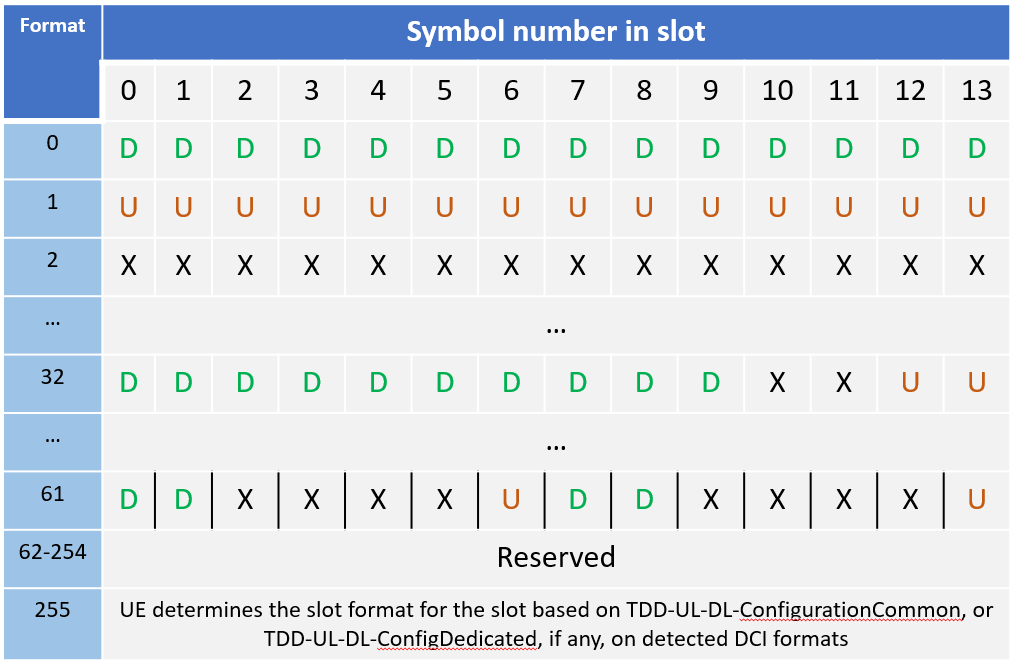
\includegraphics[width=0.6 \textwidth]{images/symbumslot.PNG}%\vspace{-6mm}
	\caption{UL/DL allocations and slot formats in 5G NR; table is abstracted from \cite{3GPP_Rel17}.} 
	\label{fig:symnumslot}
\end{figure}
As can be seen from this table, there are 62 different formats. 




%From the RAN slicing perspective \cite{num_RAN_slicing}. SINR and BER versus subcarrier index for different guardbands is obtained in the results. The main goal is to design an efficient guard band that isolates the slicing. 

%\cite{Survey_RA}

%%%%%%%%%%%%%%%%%%%%%%%%%%%%%%%%%%%%%%%%%%%%
%%%%%%%%%%%%%%%%%%%%%%%%%%%%%%%%%%%%%%%%%%%%

\section{Claudio}
%\cite{5GNR_Overview}
%5G New Radio: \\
%Physical Channels and Physical Signals \\
%Subcarrier Spacing (Tables 1,2). (Why are some spacings not supported? Used for low latency) \\
%Beam Management: 3 steps, need more info for step 3 (difference between UE reception and UE transmission) \\
%\cite{Beamforming_mMIMO}
%Benefits of beamforming \\
%mmWave beamforming uses (Section 4)\\
%Beamforming Categories (Analog/Digital/Hybrid, Adaptive...) + different arrays (2D, 3D beamforming)\\
%Need to explain what a codebook is? \\
%Need to explain SU-MIMO and MU-MIMO? \\


\section{Alex}
%%Resource Allocation and we'll compare this with the previous RA in none-HetNet, D2D communication \cite{mMIMO}
%Massive MIMO: diversite spatial \\ 
%We can use the example channel used in page 3 for demonstration \\
%mMIMO: Use of inexpensive antenna arrays instead of "expensive ultra-linear 50W amplifiers in conventional systems" (pp 3-4)\\
%ZF vs MRC in spectral efficiency \\
%Reduction of latency due to decreased fading (Need more info) \\
%Future Research Problems (if necessary) (p.8) \\
%TALK ABOUT CAPACITY??? \\



\section{Maha}
%\begin{itemize}
%		\item architecture (already done): just explain the Open RAN
%		\item low latency with claudio (Physical layer)
%		\item les futures technologies 5G (NOMA et GFDM ..)
%		\item Link layer (low latency)
%		\item Capacity and diversity
%\end{itemize}

%%%%%%%%%%%%%%%%%%%%%%%%%%%%%%%%%%%%%%%%%%%%%%%%%
%%%%%%%%%%%%%%%%%%%%%%%%%%%%%%%%%%%%%%%%%%%%%%%%%







	
\newpage
%	\IEEEQED
	\bibliographystyle{IEEEtran}
	\bibliography{biblio}
	
\end{document}